\documentclass[14pt]{extbook}
\usepackage{multicol, enumerate, enumitem, hyperref, color, soul, setspace, parskip, fancyhdr} %General Packages
\usepackage{amssymb, amsthm, amsmath, bbm, latexsym, units, mathtools} %Math Packages
\everymath{\displaystyle} %All math in Display Style
% Packages with additional options
\usepackage[headsep=0.5cm,headheight=12pt, left=1 in,right= 1 in,top= 1 in,bottom= 1 in]{geometry}
\usepackage[usenames,dvipsnames]{xcolor}
\usepackage{dashrule}  % Package to use the command below to create lines between items
\newcommand{\litem}[1]{\item#1\hspace*{-1cm}\rule{\textwidth}{0.4pt}}
\pagestyle{fancy}
\lhead{Makeup Progress Quiz 3}
\chead{}
\rhead{Version A}
\lfoot{4315-3397}
\cfoot{}
\rfoot{Fall 2020}
\begin{document}

\begin{enumerate}
\litem{
Evaluate the one-sided limit of the function $f(x)$ below, if possible.\[ \lim_{x \rightarrow 7^-} \frac{-9}{(x-7)^3}+2 \]\begin{enumerate}[label=\Alph*.]
\item \( \infty \)
\item \( f(7) \)
\item \( -\infty \)
\item \( \text{The limit does not exist} \)
\item \( \text{None of the above} \)

\end{enumerate} }
\litem{
For the graph below, find the value(s) $a$ that makes the statement true: $ \displaystyle \lim_{x \rightarrow a} f(x)$ does not exist.
\begin{center}
    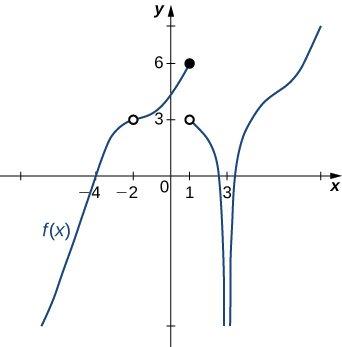
\includegraphics[width=0.5\textwidth]{../Figures/evaluateLimitGraphicallyA.png}
\end{center}
\begin{enumerate}[label=\Alph*.]
\item \( 1 \)
\item \( -2 \)
\item \( 3 \)
\item \( \text{Multiple } a \text{ make the statement true}. \)
\item \( \text{No } a \text{ make the statement true}. \)

\end{enumerate} }
\litem{
To estimate the one-sided limit of the function below as $x$ approaches 5 from the left, which of the following sets of numbers should you use?\[ \frac{\frac{5}{x} - 1}{x - 5} \]\begin{enumerate}[label=\Alph*.]
\item \( \{ 5.0000, 4.9000, 4.9900, 4.9990 \} \)
\item \( \{ 5.0000, 5.1000, 5.0100, 5.0010 \} \)
\item \( \{ 4.9000, 4.9900, 4.9990, 4.9999 \} \)
\item \( \{ 4.9000, 4.9900, 5.0100, 5.1000 \} \)
\item \( \{ 5.1000, 5.0100, 5.0010, 5.0001 \} \)

\end{enumerate} }
\litem{
Based on the information below, which of the following statements is always true?
\begin{center}
    \textit{ $f(x)$ approaches $16.016$ as $x$ approaches $0$. }
\end{center}
\begin{enumerate}[label=\Alph*.]
\item \( f(x) \text{ is close to or exactly } 16.016 \text{ when } x \text{ is close to } 0 \)
\item \( f(x) = 16.016 \text{ when } x \text{ is close to } 0 \)
\item \( f(x) = 0 \text{ when } x \text{ is close to } 16.016 \)
\item \( f(x) \text{ is close to or exactly } 0 \text{ when } x \text{ is close to } 16.016 \)
\item \( \text{None of the above are always true.} \)

\end{enumerate} }
\litem{
For the graph below, evaluate the limit: $ \displaystyle \lim_{x \rightarrow -2} f(x)$.
\begin{center}
    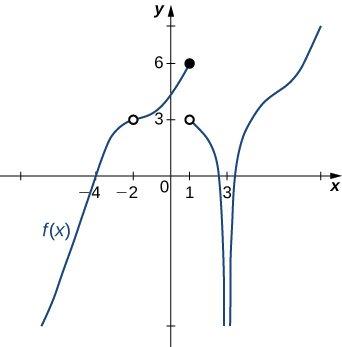
\includegraphics[width=0.5\textwidth]{../Figures/evaluateLimitGraphicallyCopyA.png}
\end{center}
\begin{enumerate}[label=\Alph*.]
\item \( -2 \)
\item \( -\infty \)
\item \( 3 \)
\item \( \text{The limit does not exist} \)
\item \( \text{None of the above} \)

\end{enumerate} }
\litem{
Evaluate the one-sided limit of the function $f(x)$ below, if possible.\[ \lim_{x \rightarrow -5^+} \frac{-1}{(x+5)^3}+5 \]\begin{enumerate}[label=\Alph*.]
\item \( -\infty \)
\item \( \infty \)
\item \( f(-5) \)
\item \( \text{The limit does not exist} \)
\item \( \text{None of the above} \)

\end{enumerate} }
\litem{
To estimate the one-sided limit of the function below as $x$ approaches 9 from the left, which of the following sets of numbers should you use?\[ \frac{\frac{9}{x} - 1}{x - 9} \]\begin{enumerate}[label=\Alph*.]
\item \( \{ 9.1000, 9.0100, 9.0010, 9.0001 \} \)
\item \( \{ 9.0000, 9.1000, 9.0100, 9.0010 \} \)
\item \( \{ 8.9000, 8.9900, 8.9990, 8.9999 \} \)
\item \( \{ 9.0000, 8.9000, 8.9900, 8.9990 \} \)
\item \( \{ 8.9000, 8.9900, 9.0100, 9.1000 \} \)

\end{enumerate} }
\litem{
Based on the information below, which of the following statements is always true?
\begin{center}
    \textit{ As $x$ approaches $\infty$, $f(x)$ approaches $16.683$. }
\end{center}
\begin{enumerate}[label=\Alph*.]
\item \( f(x) \text{ is undefined when } x \text{ is large enough}. \)
\item \( x \text{ is undefined when } f(x) \text{ is large enough}. \)
\item \( f(x) \text{ is close to or exactly } \infty \text{ when } x \text{ is large enough}. \)
\item \( f(x) \text{ is close to or exactly } 16.683 \text{ when } x \text{ is large enough}. \)
\item \( \text{None of the above are always true.} \)

\end{enumerate} }
\litem{
Evaluate the limit below, if possible.\[ \lim_{x \rightarrow 5} \frac{\sqrt{9x - 29} - 4}{2x - 10} \]\begin{enumerate}[label=\Alph*.]
\item \( 0.125 \)
\item \( 0.562 \)
\item \( \infty \)
\item \( 0.062 \)
\item \( \text{None of the above} \)

\end{enumerate} }
\litem{
Evaluate the limit below, if possible.\[ \lim_{x \rightarrow 6} \frac{\sqrt{7x - 17} - 5}{5x - 30} \]\begin{enumerate}[label=\Alph*.]
\item \( 0.529 \)
\item \( 0.100 \)
\item \( \infty \)
\item \( 0.020 \)
\item \( \text{None of the above} \)

\end{enumerate} }
\end{enumerate}

\end{document}